\documentclass[a4paper,11pt]{article}
\usepackage[T1]{fontenc}
\usepackage[utf8]{inputenc}
\usepackage{lmodern}
\usepackage{graphicx}
\graphicspath{{./img/}}
\usepackage[francais]{babel}
\title{Module d'Optique Géométrique}
\author{Rémi VAN BOXEM}

\begin{document}

\maketitle
\tableofcontents

\begin{abstract}
Comme c'est la première fois que je réalise un document grand public, laissez moi vous présenter sa composition.
\begin{itemize}
  \item \textbf{Formulaire et Résumé} : Il s'agit d'une courte partie avec l'essentiel des formules ainsi que des définitions pour comprendre rapidement la majorité du cours. Généralement cette partie est relativement courte (dépendant du nombre de formule).
  \item \textbf{Cours} : Cette partie est là pour expliquer mieux en détail le cours, ainsi que les notions importantes, il sera aggrémenté de divers exemples pour faciliter la compréhension.
  \item \textbf{Méthodes} : Dans cette section des méthodes seront énnoncés pour essayer au mieux de comprendre les exercices
  \item \textbf{QCM} : Cette section aura pour but d'évaluer vos connaissances de manière rapide et efficace sur le cours
  \item \textbf{Exercices}
  \item \textbf{Corrigés}
\end{itemize}
Vous en souhaitant bonne lecture !
\end{abstract}

\section{Formulaire et Résumé}
\subsection{Bases}

\newtheorem{form}{Formule}
\newtheorem{defi}{Définition}

\begin{defi}[Rayon Réfléchi]
Le rayon lumineux est dit \textbf{incident} avant d'avoir rencontré la surface réfléchissante, il est dit \textbf{réfléchi} après. Le point de rencontre du rayon incident et de la surface     réfléchissante est appelé \textbf{point d'incidence}. Le plan contenant le rayon incident et la normale à la surface réfléchissante au point d'incidence est dit \textbf{plan d'incidence}.
On appelle angle d'incidence l'angle orienté i pris entre la normale au point d'incidence et le rayon incident. 
\\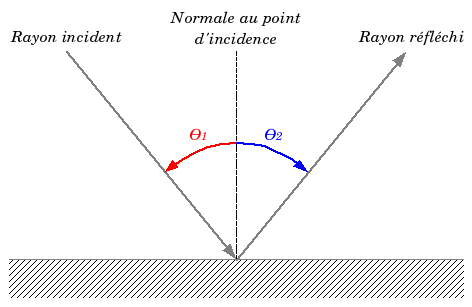
\includegraphics[scale=0.5]{Reflexion_fr.png} \centering
\end{defi}

\begin{form}[Indice de réfraction]
L'\textbf{indice de réfraction} (souvent noté $n$) est une grandeur sans dimension caractéristique d'un milieu, décrivant le comportement de la lumière dans celui-ci ; il dépend de la longueur d'onde de mesure mais aussi des caractéristiques de l'environnement (notamment pression et température). 

La définition la plus répandue pour l'indice de réfraction est qu'il est la quantité résultant du rapport entre la vitesse de la lumière $c$ dans le vide, et la vitesse de phase $v$ de la lumière dans ce milieu : $$n=\frac{c}{v}$$
A titre d'information : $n_{air}=n_{vide}=1$, $n_{eau} \approx 1,33$ et $n_{verre} \approx 1,5$
\end{form}
\begin{form}[Relation de Snell Descartes]
  La relation de \textbf{Snell Descartes} est :
  $$n_{1}*\sin(\theta_{1})=n_{2}*\sin(\theta_{2})$$
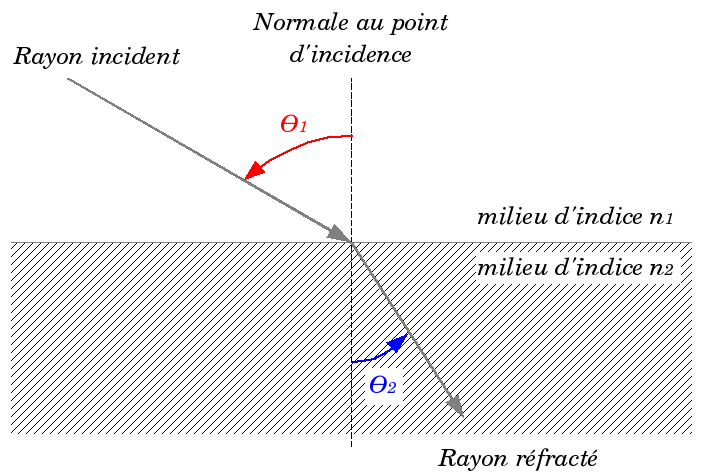
\includegraphics[scale=0.5]{Refraction_fr.png} \centering
\end{form}
\begin{defi}[Rappel : Cercle Trigonométrique]
Cercle trigonométrique et angles remarquables.
\\\centering 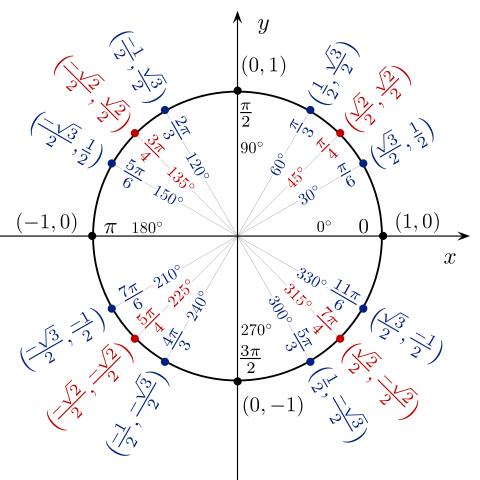
\includegraphics[scale=0.5]{trigo.png}
\end{defi}
\begin{defi}[Objet, image réelle, image virtuelle]
L'objet est souvent le sujet principal : une source lumineuse, une diapositive éclairée, un astre, une scène à photographier, etc. ; il peut s'agir de n'importe quel dispositif capable d'émettre ou de diffuser de la lumière : il s'agit alors d'objets réels. 
\\ Une image ponctuelle est le point d'intersection des rayons qui émergent du système optique.
\\Un point objet ou une image sont réels si tous les rayons au point d'intersection sont réels. En revanche, si au moins un rayon est virtuel, alors l'objet ou l'image sont virtuels.
\begin{figure}[h]
\caption{Objet réel et image réelle recueillie sur un écran}
\centering
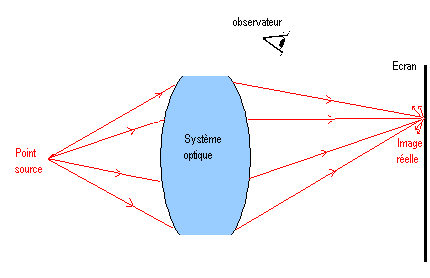
\includegraphics[width=0.5\textwidth]{Sys_optique2}
\end{figure}
\begin{figure}[h]
\caption{Objet réel et image virtuelle visible par l'œil d'un observateur placé dans le faisceau.}
\centering
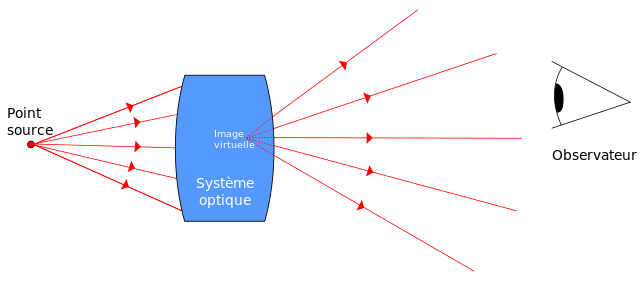
\includegraphics[width=0.5\textwidth]{Sys_optique_virt}
\end{figure}

\end{defi}
\begin{defi}[Relation de Conjugaison]
Une relation de conjugaison ou formule de conjugaison est une formule mathématique reliant la position d'un objet à celle de son image par un système optique.
\begin{figure}[h]
  \caption{Exemple de points conjugués pour un système centré.}
  \centering
  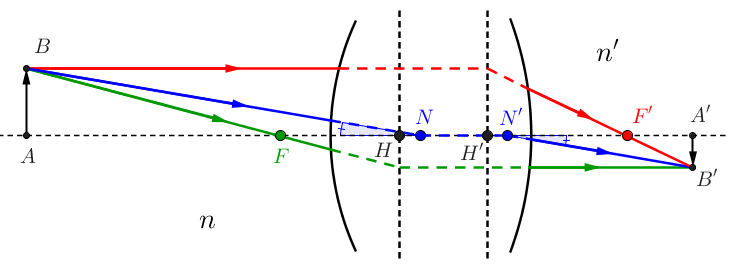
\includegraphics[width=0.5\textwidth]{Système_centré_02}
\end{figure}
\end{defi}
\begin{form}[Relation de conjugaison du miroir plan]
L'image d'un objet par un miroir plan est le symétrique orthogonal de l'objet par rapport au plan du miroir.

C'est une image virtuelle, qui ne peut être recueillie sur un écran.

L'image et l'objet sont de même taille et inversés (l'image d'une main droite est une main gauche).

Le miroir plan est le seul système optique qui soit rigoureusement stigmatique en tout point.

En pratique la réflexion par un dioptre plan (vitre, eau parfaitement calme) fournit une image identique à celle d'un miroir plan.
\begin{figure}[h]
  \caption{Image donnée par un miroir plan}
  \centering
  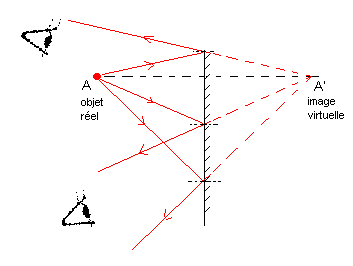
\includegraphics[width=0.5\textwidth]{Miroir_plan1}
\end{figure}
  \\ La relation de conjugaison du miroir plan est $$\overline{SA}=-\overline{SA'}$$
\end{form}
\begin{form}[Relation de conjugaison du dioptre plan]
$$\overline{SA'}=\frac{n'}{n}\overline{SA}$$
\end{form}
\begin{defi}[Réflexion totale]
Le phénomène de réflexion totale survient lorsqu'un rayon lumineux arrive sur la surface de séparation de deux milieux d'indices optiques différents avec un angle d'incidence supérieur à une valeur critique : il n'y a alors plus de rayon réfracté transmis et seul subsiste un rayon réfléchi.

Ce phénomène n'intervient que lorsque le rayon lumineux incident se trouve dans un milieu d'indice de réfraction plus grand que l'éventuel rayon réfracté.

Sur le schéma ci-contre, l'angle $\theta_1$ est plus petit que l'angle limite et le rayon rouge est à la fois réfléchi et réfracté. Pour le rayon bleu incident selon l'angle $\theta_2$ supérieur à l'angle critique, il y a réflexion totale. La mesure de l'angle limite permet ainsi de connaître le rapport des indices de réfraction des deux matériaux.
\begin{figure}[h]
  \caption{Réflexion et réfraction sur un dioptre d'indices $n_1$ et $n_2$ $(n_1 > n_2)$. Le faisceau de lumière d'angle $\theta_2$ est totalement réfléchi, tandis que celui avec un angle $\theta_1$ est réfléchi et réfracté.}
  \centering
  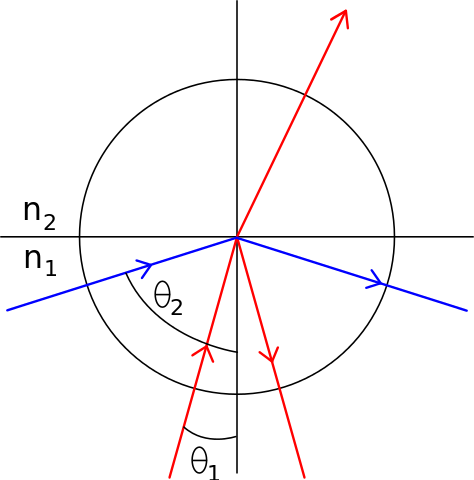
\includegraphics[width=0.5\textwidth]{Réflexion_totale}
\end{figure}
\\ La valeur $\theta_2$ limite est la valeur pour laquelle $\frac{n_1}{n_2}*\sin(\theta_1)=1$ et de cette équation, on en déduit alors la valeur de l'angle d'incidence $\theta_1$ limite correspondant : $\theta_1 = \arcsin(\frac{n_2}{n_1})$
\end{defi}
\subsection{Miroirs sphériques}
\begin{defi}[Relations de Gauss]
On dit que le miroir est dans les conditions de Gauss si les rayons incidents sont paraxiaux (autrement dit, s'ils frappent le miroir très près du sommet en faisant un angle très petit avec l'axe du miroir).

\textbf{Points et rayons particuliers :}
\begin{itemize}
\item un rayon passant par le foyer F est réfléchi parallèlement à l'axe optique ;
\item un rayon incident parallèle à l'axe optique est réfléchi en passant par le foyer F ;
\item un rayon passant par le centre de la sphère C est réfléchi sur lui-même ;
\item un rayon passant par le sommet S du miroir est réfléchi avec le même angle par rapport à l'axe optique ;
\item avec les hypothèses de Gauss (petits angles), tout rayon passant par B passe par son image B', soit réellement si B est devant le miroir, soit virtuellement si B est derrière le miroir.
\begin{figure}[h]
  \caption{Miroir sphérique concave hors des conditions de Gauss : les rayons émergents ne convergent pas.}
  \centering
  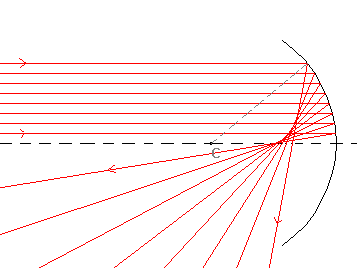
\includegraphics[width=0.5\textwidth]{miroirspheriqueconc}
\end{figure}
\end{itemize}
\end{defi}

\begin{defi}[Miroir concave, miroir convexe]
Miroir convexe : la surface réfléchissante est du côté opposé du centre de la sphère, la réflexion se fait vers l’extérieur de la sphère.
\begin{figure}[h]
  \caption{Miroir convexe : si l'objet est réel, l'image est plus petite}
  \centering
  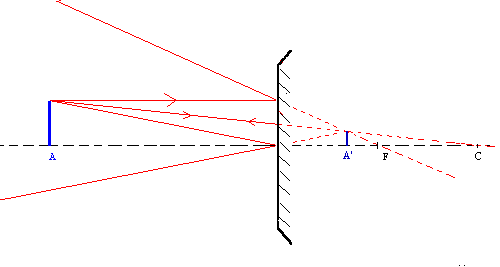
\includegraphics[width=0.5\textwidth]{miroirconvexe}
\end{figure}

\begin{figure}[h]
  \caption{Miroir concave : l'image est agrandie}
  \centering
  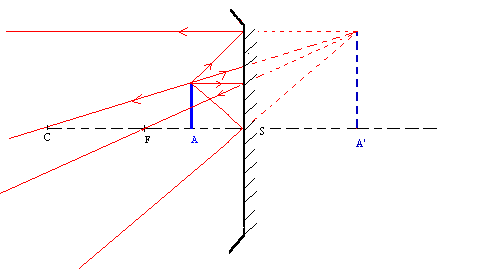
\includegraphics[width=0.5\textwidth]{miroirconcave1}
\end{figure}

\begin{figure}[h]
  \caption{Miroir concave : l'image est plus petite et inversée}
  \centering
  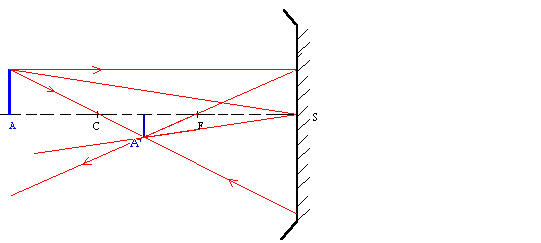
\includegraphics[width=0.5\textwidth]{miroirconcave2}
\end{figure}

\end{defi}
\subsection{Lentilles minces}
Une lentille mince est une lentille dont l'épaisseur reste faible devant les rayons de courbure de ses faces ainsi que devant la différence de ces rayons, contrairement aux lentilles épaisses.
\begin{figure}[h]
  \caption{Exemple géométrique comportant une lentille mince convergente. L'objet AB a pour image A'B'.}
  \centering
  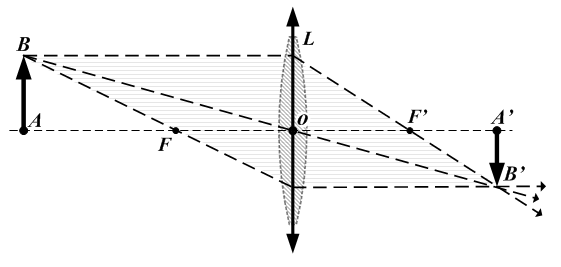
\includegraphics[width=0.5\textwidth]{ThinLens}
\end{figure}
\subsubsection{Propriétés}
Dans ce cas de la lentille mince, les distances du plan focal objet au centre optique $(\overline{FO})$ et du centre optique au plan focal image $(\overline{OF'})$, telles indiquées sur la figure sont égales. $f'=\overline{OF'}$ est la distance focale de la lentille.
\\On appelle alors vergence d'une lentille la quantité $C=\frac{1}{f'}$. Son unité est la dioptrie (symbole $\delta$).
\subsubsection{Formules de conjugaison}
Les formules de conjugaison de Descartes donnent une relation entre les positions sur l'axe optique d'un objet et de son image par rapport au centre optique.

Lorsque les conditions de Gauss sont vérifiées, l'image d'un objet perpendiculaire à l'axe optique est perpendiculaire à l'axe optique : on peut ainsi déterminer la position de l'image d'un point B hors d'axe en considérant l'image du point A qui est la projection de B sur l'axe optique (voir les images ci-dessous).

Notons également qu'un objet :
\begin{itemize}
\item à l'infini donnera une image dans le plan focal image de la lentille ;
\item placé à $2.f$ (deux fois la distance focale objet) donnera une image inversée identique à l'objet (grandissement : $\gamma  = -1$) située à $2.f'$ (deux fois la distance focale image) ;
\item au-delà de la distance focale objet donnera une image réelle ;
\item dans le plan focal objet donnera une image à l'infini ;
\item entre le foyer image et le centre optique de la lentille donnera une image virtuelle.
\end{itemize}
\subsubsection{Constructions optiques}
Pour effectuer des constructions sur un schéma optique, on considère 3 rayons particuliers :
\begin{itemize}
\item le rayon passant par le centre optique n'est pas dévié (si le milieu est le même de chaque côté de la lentille) ;
\item le rayon parallèle à l'axe avant la lentille est dévié et le rayon sortant passe par le foyer image ;
\item le rayon passant par le foyer objet avant la lentille est dévié et ressort parallèle à l'axe.
\end{itemize}
Ceci permet de construire l'image $A'B'$ d'un petit objet $AB$ perpendiculaire à l'axe optique.
\paragraph{Construction des rayons pour une lentille divergente}
\begin{figure}[h]
  \caption{Schéma lentille mince divergente : foyer image}
  \centering
  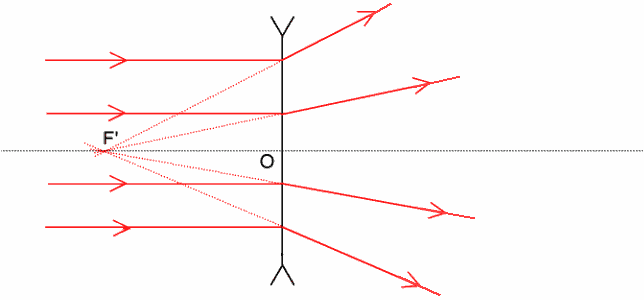
\includegraphics[width=0.5\textwidth]{lentillemincediv1}
\end{figure}
\begin{figure}[h]
  \caption{Schéma lentille mince convergente : foyer objet}
  \centering
  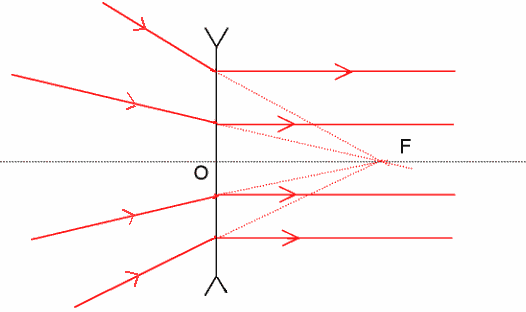
\includegraphics[width=0.5\textwidth]{lentillemincediv2}
\end{figure}
\paragraph{Construction des rayons pour une lentille convergente}
\begin{figure}[h]
  \caption{Construction de l'image de B par les rayons pour une lentille convergente}
  \centering
  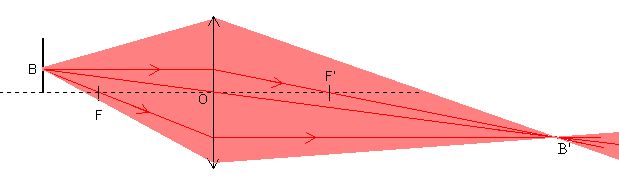
\includegraphics[width=0.5\textwidth]{Lc7}
\end{figure}
\begin{figure}[h]
  \caption{Schéma lentille mince convergente : schématisation, rayons particuliers}
  \centering
  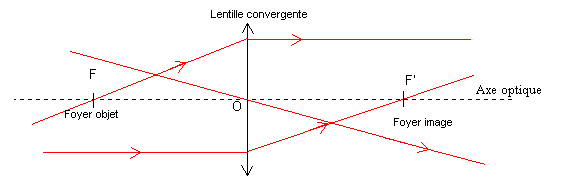
\includegraphics[width=0.5\textwidth]{Lc4}
\end{figure}
\begin{figure}[h]
  \caption{Construction de l'image de AB par les rayons pour une lentille convergente}
  \centering
  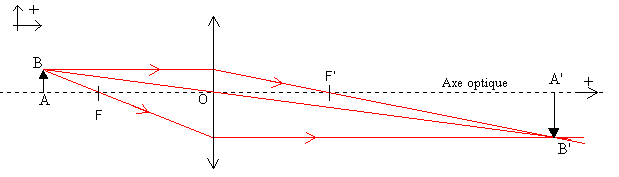
\includegraphics[width=0.5\textwidth]{Lc5}
\end{figure}
Comme le montre la zone rouge sur la première image, tous les rayons issus de $B$ passant par la lentille convergent en $B'$. Les 3 rayons particuliers permettent de déterminer l'emplacement de $B'$.

Il faut également noter que des rayons parallèles se coupent au même foyer secondaire. Pour un rayon quelconque, il est ainsi possible de tracer sa propagation après la lentille, en considérant le rayon parallèle qui passe par l'axe optique (et n'est donc pas dévié) : les deux rayons se coupent au niveau du plan focal image.

\newpage
\subsection{Instruments d'optique}
\begin{defi}[Punctum proximum, punctum remotum]
\textbf{Punctum proximum :} le point le plus proche que l’on peut voir net correspondant
au maximum de contraction du cristallin (Environ $10$ ou $20$ cm)
\\\textbf{Punctum remotum :} le point le plus éloigné que l’on peut voir net
Pour un œil emmétrope, c’est l’infini 
\end{defi}
\end{document}
